\section{Frontend: Actualizaciones Reactivas y Consumo en Tiempo Real}
\label{sec:s3_frontend}

El frontend integra las experiencias diferenciales del producto: pipeline Kanban del reclutador,
dashboards analíticos, chat con presencia y el CV Studio. La Figura~\ref{fig:s3_kanban} esquematiza
el pipeline de Talent Discovery.\par

\begin{figure}[!ht]
    \centering
    \begin{tikzpicture}[
        col/.style={draw=colorPrimario, fill=headerTabla, thick, rounded corners=3pt,
            text width=2.1cm, align=center, minimum height=2.2cm, font=\sffamily\scriptsize},
        card/.style={draw=grisISO, fill=white, rounded corners=2pt, text width=1.8cm,
            align=center, minimum height=0.5cm, font=\sffamily\tiny},
        rel/.style={-{Latex[length=1.6mm]}, grisISO}
    ]
        \node[col] (c1) {};
        \node[col, right=0.4cm of c1] (c2) {};
        \node[col, right=0.4cm of c2] (c3) {};
        \node[col, right=0.4cm of c3] (c4) {};
        \node[font=\sffamily\tiny\color{colorPrimario}, above=1pt of c1] {Nuevo};
        \node[font=\sffamily\tiny\color{colorPrimario}, above=1pt of c2] {Contactado};
        \node[font=\sffamily\tiny\color{colorPrimario}, above=1pt of c3] {Entrevista};
        \node[font=\sffamily\tiny\color{colorPrimario}, above=1pt of c4] {Oferta};
        \node[card] at ([yshift=0.6cm]c1.center) {Candidato A};
        \node[card] at ([yshift=0.6cm]c2.center) {Candidato B};
        \draw[rel] (c1)--(c2); \draw[rel] (c2)--(c3); \draw[rel] (c3)--(c4);
    \end{tikzpicture}
    \caption{Pipeline Kanban de Talent Discovery (\textit{drag \& drop} con dnd-kit).}
    \label{fig:s3_kanban}
\end{figure}

\subsection{Clientes WebSocket para Eventos Asíncronos}
\label{ssec:s3_fe_ws}
El frontend integra clientes de Supabase Realtime para la escucha y el envío de eventos
asíncronos: mensajes de chat, presencia y notificaciones (Sonner). El \comando{cvStudioStore} y el
editor \textbf{Monaco} dan vida al CV Studio con el asistente de IA, y los datos geográficos se
muestran con \textbf{Leaflet}.

\begin{itemize}[noitemsep]
    \item \textbf{Suscripción a canales:} altas/bajas controladas al montar/desmontar la vista.
    \item \textbf{Reconexión:} reintentos con preservación de idempotencia para no duplicar mensajes.
    \item \textbf{Presencia:} indicador en línea/desconectado por usuario.
\end{itemize}

\subsection{Actualización Fluida de la UI sin Recarga}
\label{ssec:s3_fe_reactiva}
La interfaz se actualiza sin recargar la página: paneles colaborativos, alertas emergentes y el
pipeline Kanban con \textit{drag \& drop} (dnd-kit). Los dashboards del reclutador usan
\textbf{Recharts} (funnel, radar de skills, KPIs). La Figura~\ref{fig:s3_dashboard} muestra el
dashboard analítico.

\begin{figure}[!ht]
    \centering
    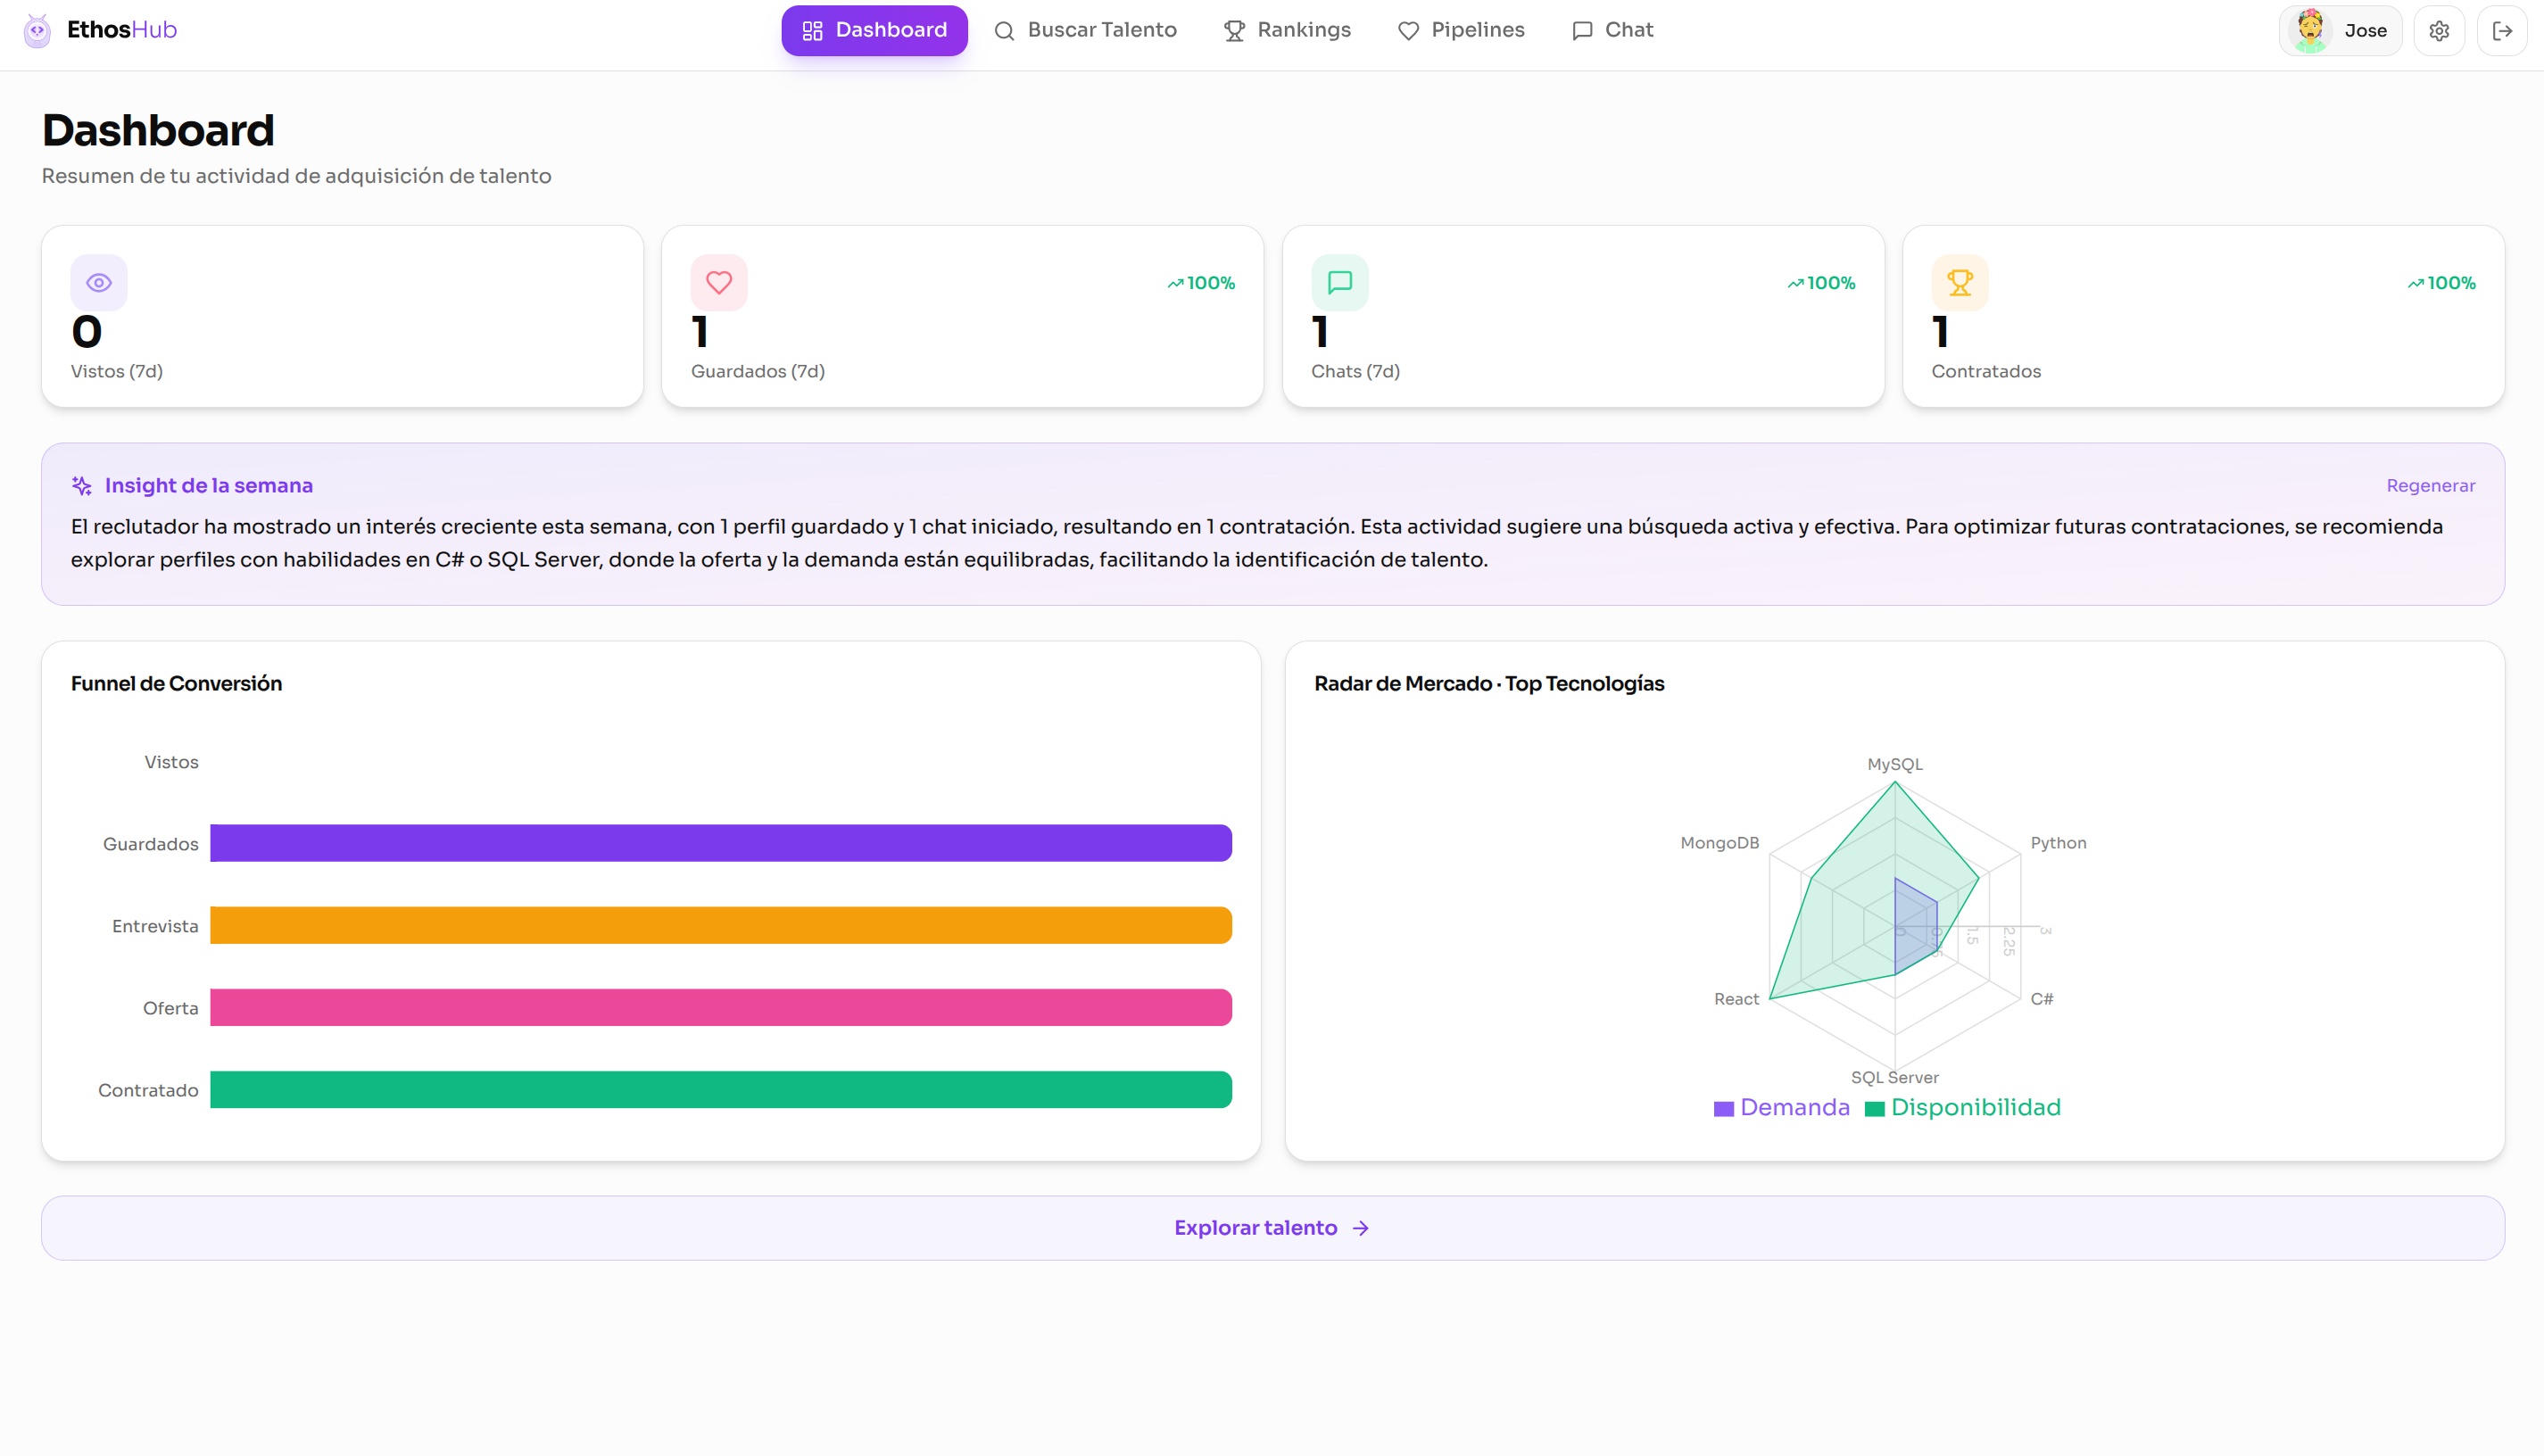
\includegraphics[width=0.7\textwidth]{assets/img/ethoshub/dashboard.png}
    \caption{Dashboard analítico del reclutador (Recharts).}
    \label{fig:s3_dashboard}
\end{figure}

\begin{itemize}[noitemsep]
    \item \textbf{Kanban:} arrastrar y soltar candidatos entre fases del pipeline.
    \item \textbf{Match ring:} indicador visual de afinidad del candidato.
    \item \textbf{Insights IA:} cuatro modos de análisis asistido por Gemini.
    \item \textbf{CV Studio:} edición en Monaco, compilación a PDF y chat con la IA.
\end{itemize}

\subsection{Stores, Servicios y Librerías Avanzadas}
\label{ssec:s3_fe_stores}
Las funcionalidades avanzadas integran las librerías y \textit{stores} de la
tabla~\ref{tab:s3_fe_stores}.

\begin{table}[!ht]
    \centering
    \renewcommand{\arraystretch}{1.3}
    \fontsize{9}{10.8}\selectfont\sffamily
    \begin{tabularx}{\textwidth}{|l|X|}
        \hline
        \rowcolor{colorPrimario}
        \textcolor{white}{\textbf{Elemento}} & \textcolor{white}{\textbf{Responsabilidad}} \\ \hline
        \comando{cvStudioStore} / \comando{cvStudioService} & Documento de CV, asistente IA y compilación. \\ \hline
        \rowcolor{grisTecnico}
        \comando{projectsStore} / \comando{fileService} & Vitrina y subida de evidencias. \\ \hline
        \comando{connectionsStore} & Conexiones URL-first a apps externas. \\ \hline
        \rowcolor{grisTecnico}
        \comando{dashboardService} & Funnel, radar y KPIs del reclutador. \\ \hline
        \comando{@dnd-kit/*} & \textit{Drag \& drop} del pipeline Kanban. \\ \hline
        \rowcolor{grisTecnico}
        Recharts / Leaflet & Gráficas analíticas y mapas. \\ \hline
        Monaco Editor & Editor de código del CV Studio. \\ \hline
        \rowcolor{grisTecnico}
        \comando{@supabase/supabase-js} & Canales Realtime de chat y presencia. \\ \hline
    \end{tabularx}
    \caption{Stores, servicios y librerías de las funcionalidades avanzadas (Sprint 3).}
    \label{tab:s3_fe_stores}
\end{table}

La suscripción a canales Realtime se gestiona en el ciclo de vida del componente: se abre al
montar la vista y se cierra al desmontarla, evitando fugas de \textit{listeners}; la reconexión
preserva la idempotencia descrita en la Sección~\ref{ssec:s3_be_realtime}.

\clearpage
